\documentclass[convert]{standalone}

\usepackage{tikz}
\usepackage{graphicx}
\pagestyle{empty}

% INT_AY22_L28-Fig14_B_fields_w_paths.png

\begin{document}
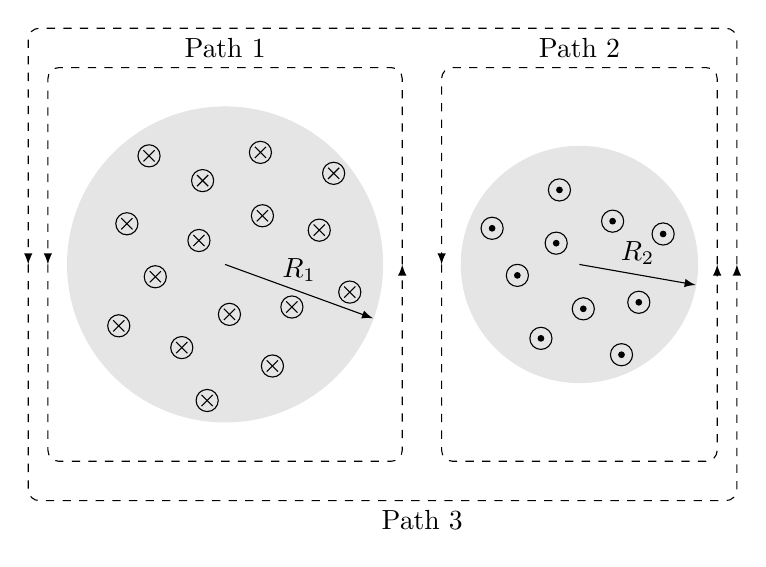
\begin{tikzpicture}[> = latex]

	% Magnetic field regions
	
	\filldraw [gray!20] (-2.5, 0) circle (2 cm);
	\filldraw [gray!20] (2, 0) circle (1.5 cm);
	
	% Radius indicators
	
	\draw [->] (-2.5, 0) -- node [above] {$R_1$} ++ (-20 : 2);
	\draw [->] (2, 0) -- node [above] {$R_2$} ++ (-10 : 1.5);
	
	% Put field indicators in Fermat spiral pattern
	
	\foreach \n in {1, 2, ..., 16}
	{
		\draw (-2.5, 0) ++ (137.5 * \n : {0.45 * sqrt(\n)}) ++ (0.071, 0.071) -- ++ (-0.142, -0.142);
		\draw (-2.5, 0) ++ (137.5 * \n : {0.45 * sqrt(\n)}) ++ (0.071, -0.071) -- ++ (-0.142, 0.142);
		\draw (-2.5, 0) ++ (137.5 * \n : {0.45 * sqrt(\n)}) circle (4 pt);
	}
	
	\foreach \n in {1, 2, ..., 10}
	{
		\filldraw (2, 0) ++ (137.5 * \n : {0.4 * sqrt(\n)}) circle (1 pt);
		\draw (2, 0) ++ (137.5 * \n : {0.4 * sqrt(\n)}) circle (4 pt);
	}
	
	% Draw paths
	
	\draw [dashed, rounded corners, ->] (-0.25, 0) -- (-0.25, 2.5) -- node [above] {Path 1} (-4.75, 2.5) -- (-4.75, 0);
	\draw [dashed, rounded corners, ->] (-4.75, 0) -- (-4.75, -2.5) -- (-0.25, -2.5) -- (-0.25, 0);
	
	\draw [dashed, rounded corners, ->] (0.25, 0) -- (0.25, -2.5) -- (3.75, -2.5) -- (3.75, 0);
	\draw [dashed, rounded corners, ->] (3.75, 0) -- (3.75, 2.5) -- node [above] {Path 2} (0.25, 2.5) -- (0.25, 0);
	
	\draw [dashed, rounded corners, ->] (4, 0) -- (4, 3) -- (-5, 3) -- (-5, 0);
	\draw [dashed, rounded corners, ->] (-5, 0) -- (-5, -3) -- node [pos = 0.556, below] {Path 3} (4, -3) -- (4, 0);
	
\end{tikzpicture}
\end{document}